\documentclass{article} % For LaTeX2e
\usepackage{nips12submit_e,times}
%\documentstyle[nips12submit_09,times,art10]{article} % For LaTeX 2.09

% For figures
\usepackage{multirow}

\usepackage{graphicx} % more modern
%\usepackage{epsfig} % less modern
\usepackage{subfigure} 

% \usepackage{natbib} % For citations
\usepackage{subfigure}
\usepackage{algorithm,algorithmic} % For algorithms

% As of 2011, we use the hyperref package to produce hyperlinks in the
% resulting PDF.  If this breaks your system, please commend out the
% following usepackage line and replace \usepackage{icml2013} with
% \usepackage[nohyperref]{icml2013} above.
\usepackage{hyperref}
% \nocite{*}
\usepackage[normalem]{ulem}
\usepackage{sidecap}

% Packages hyperref and algorithmic misbehave sometimes.  We can fix
% this with the following command.
\newcommand{\theHalgorithm}{\arabic{algorithm}}

% jovo added stuff
\newcommand{\iid}{\overset{iid}{\sim}}
\newcommand{\mbX}{\mathbf{X}}
\newcommand{\mbY}{\mathbf{Y}}
\newcommand{\Real}{\mathbb{R}}
\providecommand{\mh}[1]{\hat{#1}}
\providecommand{\mb}[1]{\boldsymbol{#1}}
\providecommand{\mc}[1]{\mathcal{#1}}
\providecommand{\mt}[1]{\widetilde{#1}}
\newcommand{\from}{{\ensuremath{\colon}}}  % :
\usepackage{amsmath,amssymb,amsfonts}
\newcommand{\conv}{\rightarrow}

\newcommand{\efoo}{\end{footnotesize}}
\newcommand{\bfoo}{\begin{footnotesize}}
\renewcommand{\labelenumi}{\theenumi}
\floatname{algorithm}{Procedure}
\renewcommand{\algorithmicrequire}{\textbf{Input:}}
\renewcommand{\algorithmicensure}{\textbf{Output:}}
\floatname{algorithm}{Pseudocode}
\providecommand{\norm}[1]{\left \lVert#1 \right  \rVert}
\newcommand{\T}{^{\ensuremath{\mathsf{T}}}}           % transpose


% Employ the following version of the ``usepackage'' statement for
% submitting the draft version of the paper for review.  This will set
% the note in the first column to ``Under review.  Do not distribute.''

% Employ this version of the ``usepackage'' statement after the paper has
% been accepted, when creating the final version.  This will set the
% note in the first column to ``Proceedings of the...''
% \usepackage[accepted]{icml2013}

% jovo additions
\usepackage{color}
\newcommand{\jovo}[1]{{\color{magenta}{\it #1}}}
\newcommand{\msd}{Ms.~Deeds}
% \newcommand{\Real}{\mathbb{R}}
\newcommand{\ZZ}{\mathbb{Z}}
\newcommand{\II}{\mathbb{I}}
\usepackage{color}
\newcommand{\dd}[1]{{\color{blue}{\it #1}}}
\newtheorem{theorem}{Theorem}%[section]
\newtheorem{lemma}[theorem]{Lemma}
\newtheorem{proposition}[theorem]{Proposition}
\newtheorem{corollary}[theorem]{Corollary}
\newtheorem{result}[theorem]{Result}
\newtheorem{definition}[theorem]{Definition}
\providecommand{\mtc}[1]{\widetilde{\mathcal{#1}}}

\setlength{\parsep}{0pt}
\setlength{\headsep}{0pt}
\setlength{\topskip}{0pt}
\setlength{\topmargin}{0pt}
\setlength{\topsep}{0pt}
\setlength{\partopsep}{0pt}

\setlength{\parskip}{2pt}
\parindent 10pt

\usepackage[compact]{titlesec}
% \titlespacing{\section}{20pt}{*0}{*0}
% \titlespacing{\subsection}{5pt}{*0}{*0}
% \titlespacing{\subsubsection}{5pt}{*0}{*0}

% The \icmltitle you define below is probably too long as a header.
% Therefore, a short form for the running title is supplied here:
\title{Multiscale Dictionary Learning for \\ Estimating Conditional Distributions}


%\nipsfinalcopy % Uncomment for camera-ready version

\begin{document}
\renewcommand{\theenumi}{(\roman{enumi})}%


\maketitle

\begin{abstract}
Nonparametric estimation of the conditional distribution of a response given high-dimensional features is a challenging problem.  In many settings it is important to allow not only the mean but also the variance and shape of the response density to change flexibly with features, which are massive-dimensional with a distribution concentrated near a lower-dimensional subspace or manifold.  We propose a  multiscale model based on a novel stick-breaking prior placed on the dictionary weights.  The algorithm scales efficiently to massive numbers of features, and can be implemented efficiently with slice sampling.  State of the art predictive performance is demonstrated for toy examples and a real data application.
\end{abstract}

% \tableofcontents

\section{Introduction}


% opening
Massive datasets are becoming a ubiquitous by-product of modern scientific and industrial applications. These data present statistical and computational challenges for machine learning because many previously developed approaches do not scale-up sufficiently.  Specifically, challenges arise because of the ultrahigh-dimensionality and relatively low sample size (the ``large p, small n'' problem).  Parsimonious models for such big data assume that the density in the ambient dimension concentrates around a lower-dimensional (possibly nonlinear) subspace.  Indeed, a plethora of methodologies are emerging to estimate such lower-dimensional manifolds from high-dimensional data \cite{Manifold, Maggioni}.  

We are interested in using such lower-dimensional embeddings to obtain estimates of the conditional distribution of some target variable(s).  This \emph{conditional density estimation} setting arises in a number of important application areas, including neuroscience, genetics, and video processing.  For example, one might desire automated estimation of a predictive density for a continuous neurologic { phenotype} of interest, such as intelligence or a creativity, on the basis of available data for a patient including neuroimaging.  The challenge is to estimate the probability density function of the phenotype {\em nonparametrically} based on an $\approx 10^6$ dimensional image of the subject's brain.  It is crucial to avoid parametric assumptions on the density, such as Gaussianity, while allowing the density to change flexibly with predictors.  Otherwise, one can obtain misleading predictions and poorly characterize predictive uncertainty.

There is a rich machine learning and statistical literature on conditional density estimation of a response $y \in \mathcal{Y}$ given a set of features (predictors) $x=(x_1, x_2, \ldots, x_p)\in \mathcal{X}$. Common approaches include hierarchical mixtures of experts \cite{mixtureexperts,jiang1999}, kernel methods \cite{fan1996,fanyim2004,holmes2010,fu2011}, Bayesian finite mixture models \cite{nott2012,tran2012,norets2012} and Bayesian nonparametrics 
\cite{griffin06, dunson2007, DunsonPark, chung2009, tokdar2010}.  

% challenge
However, there has been limited consideration of scaling to large $p$ settings, with the variational Bayes approach of \cite{tran2012} being a notable exception. For dimensionality reduction, Tran et al. follow a greedy variable selection algorithm.  Their approach does not scale to the sized applications we are interested in. For example, in a problem with $p=1,000$ and $n=500$, they reported a CPU time of 51.7 minutes for a single analysis.  We are interested in problems with  $p$ having many more orders of magnitude, requiring a faster computing time while also accommodating flexible non-linear dimensionality reduction (variable selection is a limited sort of dimension reduction).  To our knowledge, there are no nonparametric density regression competitors to our approach, which maintain a characterization of uncertainty in estimating the conditional densities; rather, all sufficiently scalable algorithms provide point predictions and/or rely on restrictive assumptions such as linearity.  

In big data problems, scaling is often accomplished using divide-and-conquer techniques. 
% Well known examples are classification and regression trees (CART) \cite{CART} and multivariate adaptive regression splines (MARS) \cite{MARS}. These algorithms fit surfaces to data by explicitly dividing the input space into a nested sequence of regions, and by fitting simple surfaces  within these regions. Though these methods are appealing in providing a simple, flexible and interpretable mechanism of dimension reduction, it is well known that single tree estimates commonly have high variance and poor performance.  There is a rich literature proposing improvements based on bagging \cite{Bagging}, boosting \cite{Boosting} and random forests \cite{RandomForest}. Though these algorithms can substantially improve mean square error performance, computation can be expensive and performance degrades as dimensionality $p$ increases.
% 
% In fact, 
a significant downside of many divide-and-conquer algorithms is their poor scalability to high dimensional predictors. As the number of features increases, the problem of finding the best splitting attribute becomes intractable so that CART, MARS and multiple trees models cannot be efficiently applied. Similarly, mixture of experts models become computationally demanding, since both mixture weights and dictionary densities are predictor dependent. In an attempt to make mixtures of experts more efficient, sparse extensions relying on different variable selection algorithms have been proposed \cite{SparseMoF}. However, performing variable selection in high dimensions is effectively intractable: algorithms need to efficiently search for the best subsets of predictors to include in weight and mean functions within a mixture model, an NP-hard problem.

% approach
 In order to efficiently deal with massive datasets, we propose a novel multiscale approach which starts by learning a multiscale dictionary of densities. This tree is efficiently learned in a first stage using a fast and scalable graph partitioning algorithm applied to the high-dimensional observations \cite{metis}.  Expressing the conditional densities $F_{Y|X}$ for each $x \in \mathcal{X}$ as a convex combination of coarse-to-fine scale dictionary densities, the learning problem in the second stage estimates the corresponding multiscale probability tree.  This is accomplished in a Bayesian manner using a novel multiscale stick-breaking process, which allows the data to inform about the optimal bias-variance tradeoff; weighting coarse scale dictionary densities more highly decreases variance while adding to bias.  This results in a model that borrows information across different resolution levels and reaches a good compromise in terms of the bias-variance tradeoff. We show that the algorithm scales efficiently to millions of features. 

% \vspace{-25pt}
\section{Setting} \label{sec:setting}
% \vspace{-25pt}
Let $X \from \Omega \to \mc{X} \subseteq \Real^p$ be a 
$p$-dimensional Euclidean vector-valued predictor random variable, taking values $x \in \mc{X}$, with a marginal probability distribution $F_X$.  
Similarly, let $Y \from \Omega \to \mc{Y}$ 
be a $\mc{Y}$-valued target random variable, taking values $y \in \mc{Y}$, with a marginal probability distribution $F_Y$ (we will specify specific forms of $\mc{Y}$, e.g., $\mc{Y} \subseteq \Real^q$, below).  We assume that the pair $(X,Y)$ is sampled from a joint distribution, $F_{X,Y} \in \mc{F}$. Let $F_{Y|X}$ denote the conditional (cumulative) distribution, and $f_{y|x}$ denote the conditional (probability) density.

For inferential expedience, we  posit the existence of  a latent random variable $\mb{\eta} \from \Omega \to \mc{M} \subseteq \mc{X}$, where $\mc{M}$ is only $d$ ``dimensional'' and $d \ll p$.   
Note that $\mc{M}$ need not be a linear subspace of $\mc{X}$, rather, $\mc{M}$ could be, for example,  a union or affine subspaces, or a smooth compact Riemannian manifold.  Regardless of the nature of $\mc{M}$, we assume that we can approximately decompose the joint distribution as follows,  $F_{X,Y,\mb{\eta}}=F_{X,Y|\mb{\eta}}F_{\mb{\eta}} = F_{Y|X, \mb{\eta}} F_{X | \mb{\eta}} F_{\mb{\eta}} \approx F_{X|\mb{\eta}} F_{Y|\mb{\eta}} F_{\mb{\eta}}$.  In  words, we assume that the \emph{signal} approximately concentrates around a low-dimensional latent space, $F_{Y|X,\mb{\eta}}=F_{Y|\mb{\eta}}$.  Note that this is a much less restrictive assumption than the commonplace assumption in manifold learning that the marginal distribution $F_X$ concentrates around a low-dimensional latent space. 

To provide some intuition around this model, we provide the following concrete example where the distribution of $y \in \Real$ is a Gaussian function of the coordinate $\eta \in \mc{M}$ along the swissroll, which is embedded in a high-dimensional ambient space.  Specifically, we sample the manifold coordinate, $\eta  \sim U(0,1)$.  Then the first two dimensions of $X$ are

	$X_1 = \eta \sin (\eta)$ and
	$X_2 = \eta \cos (\eta)$.
	The remaining dimensions of $X$ are sampled from a Gaussian,
$X_r \sim \mc{N}(0,1) \text{ for } r \in \{3, \ldots, p\}$.
Finally, we sample $Y$ conditionally dependent only on $\eta$: 	$Y | \eta \sim \mc{N}(\mu(\eta) ,\sigma(\eta))$.
% \begin{subequations} \label{eq:linear}
% \begin{align}
% 	Y | \eta &\sim \mc{N}(\mu(\eta) ,\sigma(\eta)) \\
% X_r &\sim \mc{N}(0,1) \text{ for } r \in \{3, \ldots, p\}, \qquad 	X_1 = \eta \sin (\eta), \qquad X_2 = \eta \cos (\eta) \\
% 	\eta  &\sim U(0,1), 
% \end{align}
% \end{subequations}
% where $\mc{N}(\mu,\sigma)$ denotes a Gaussian distribution with mean $\mu$ and standard deviation $\sigma$, and $U(0,1)$ denotes the uniform distribution on $(0,1)$.
Clearly, $Y$ is conditionally dependent on ${\eta}$, which is the low-dimensional signal manifold, of which $X$ is also a function.  In particular, $X$ lives on a swissroll embedded in a $p$-dimensional ambient space, but $Y$ is only a function of the coordinate ${\eta}$ along the swissroll $\mc{M}$. The left panels of Figure \ref{fig:swiss} depict this concrete example when $\mu(\eta)=\eta$ and $\sigma(\eta)=\eta + 1$.


\begin{figure}[htbp]
	\centering
		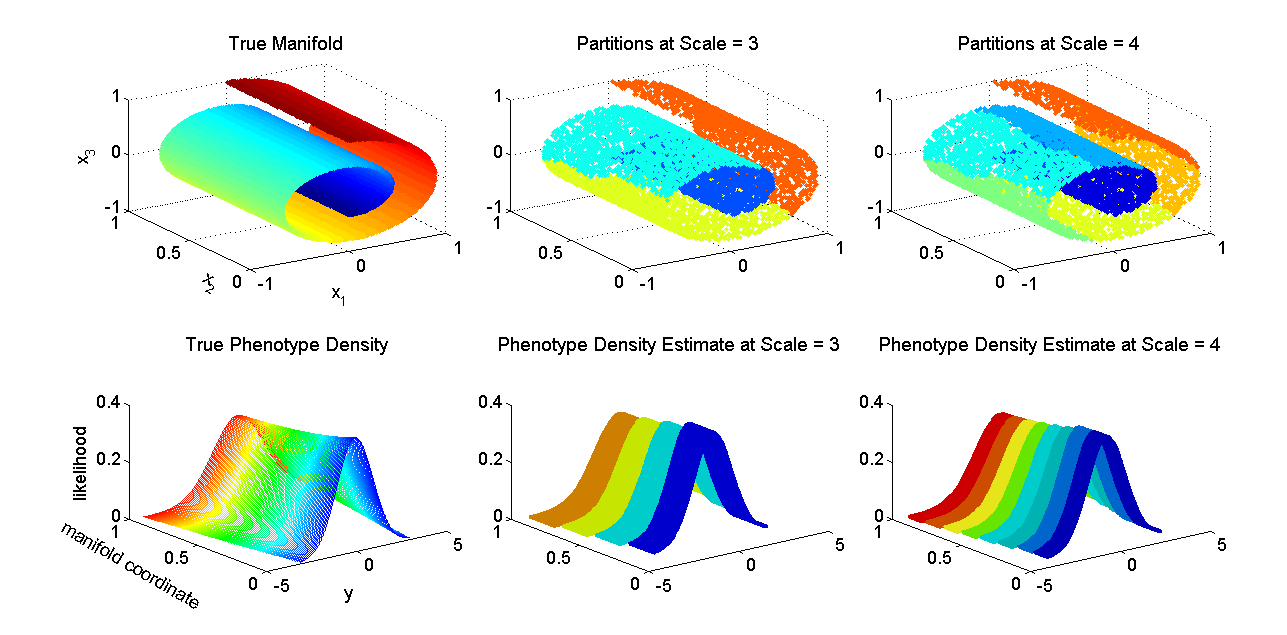
\includegraphics[width=1\linewidth]{../figs/PartitionsDensity_27MAY}
	\caption{Illustration of our generative model and algorithm on a swissroll. The top left panel shows the manifold $\mc{M}$ (a swissroll) embedded in a $p$-dimensional ambient space, where the color indicates the coordinate along the manifold, $\eta$ (only the first 3 dimensions are shown for visualization purposes). The bottom left panel shows the distribution of $Y$ as a function of $\eta$, in particular, $F_{Y|\eta}=\mc{N}({\eta},{\eta}+1)$. The middle and right panels show our estimates of $F_{Y|{\eta}}$ at scales 3 and 4, respectively, which follow from partitioning our data.  Sample size was $n=10\,000$.}
	\label{fig:swiss}
\vskip -10pt
\end{figure}


\section{Goal} \label{sec:goal}

Our goal is to develop an approach to learn about $F_{Y|X}$ from $n$ pairs of observations that we assume are sampled exchangeable from the joint distribution, $(x_i,y_i) \sim F_{X,Y} \in \mc{F}$. Let $\mc{D}^n=\{(x_i,y_i)\}_{i \in [n]}$, where $[n]=\{1,\ldots, n\}$.  More specifically, we seek to obtain a posterior over $F_{Y|X}$.  We insist that our approach satisfies several desiderata, including most importantly: (i) scales up to $p \approx 10^6$ in reasonable time,  (ii) yields good empirical results, and (iii) automatically adapts to the complexity of the data corpus.  To our knowledge, no extant approach for estimating conditional densities or posteriors thereof satisfies even our first criterion. 
%Below, we provide a general multiscale approach to this problem (\S \ref{sub:method}), followed by our specific choices (\S \ref{sub:spec}), results on simulated (\S \ref{sub:sim}) and real neuroscience (connectomics) data (\S \ref{sub:real}), and a discussion (\S \ref{sec:disc}).


\section{Methodology} \label{sec:method}

\subsection{\msd~Framework} \label{sub:method}

We propose here a general modular approach which we refer to as \uline{m}ulti\uline{s}cale \uline{d}ictionary learning for \uline{e}stimating conditional \uline{d}istribution\uline{s} (``\msd''). \msd~consists of three components: (i) a tree decomposition of the space, (ii) an embedding of the data into a lower-dimensional space,  and (iii) an assumed form of the conditional probability model. 

\paragraph{Tree Decomposition}
A tree decomposition $\tau$ yields a multiscale partition of the data or the ambient space in which the data live.
Let $(\mc{W},\rho_W, F_W)$ be a measurable metric space, where $F_W$ is a Borel probability measure, $\mc{W}$, and $\rho_W \from \mc{W} \times \mc{W} \to \Real$ is a metric on $\mc{W}$.  Let $B_r^{\mc{W}}(w)$ be the $\rho_W$-ball inside $\mc{W}$ of radius $r > 0$ centered at $w \in \mc{W}$. For example, $\mc{W}$ could be the data corpus $\mc{D}_n$, or it could be $\mc{X} \times \mc{Y}$. We define a tree decomposition as in \cite{Allard2012,ChenMaggioni12}.  A partition tree $\tau$ of $\mc{W}$ consists of a collection of cells, $\tau=\{C_{j,k}\}_{j \in \ZZ, k \in \mc{K}_j}$.  At each scale $j$, the set of cells $C_j=\{C_{j,k}\}_{k \in \mc{K}_j}$ provides a disjoint partition of $\mc{W}$ almost everywhere, and $\mc{K}_j$ is the set of partitions at scale $j$.  We define $j=0$ as the root node/cell.  For each $j > 0$,  each $C_{j,k}$ has a unique parent node $C_{j-1,k'}$ containing $C_{j,k}$, and conversely, any $C_{j,k} \subseteq C_{j-1,k'}$ is called a child of $C_{j-1,k'}$.


Let $A_{j,k}=\{k' \in \mc{K}_{j'} : j' < j$ s.t. $C_{j,k} \subseteq C_{j',k'}\}$ denote the ancestors of $C_{j,k}$, and let $D_{j,k}=\{k' \in \mc{K}_{j'} : j' > j$ s.t. $C_{j',k'} \subseteq C_{j,k}\}$ denote the descendants of $C_{j,k}$.
% Figure \ref{graph}(i) depicts a binary tree decomposition for some data (note that the tree need not be binary). 
In classical multiscale function estimation, at each scale, we would approximate the function via a mixture: $\mh{F}_j = \sum_{k \in \mc{K}_j} \omega_{j,k} \mh{F}_{j,k}$, where the $\{\omega_{j,k}\}_{j \in \mc{K}_j}$ are mixture weights \emph{within} a scale, such that $\sum_{k \in \mc{K}_j} \omega_{j,k}=1$.  Rather than choosing a scale, however, given a new observation, one can also mix \emph{across scales},  by placing a prior over scales.  In such a case, given a new observation $x$ for which we would like an estimate of $f_{y|x}$, we have the following approximation 
\begin{align}
\mh{f}_{y|x} \approx \sum_{C_{j',k'} \in A_{j,k}} \pi_{j',k'} f^{j',k'}_{y|x}	\label{eq:base}
\end{align}
where $\pi_{j',k'}$ are weights \emph{across scales} such that $\sum_{C_{j',k'} \in A_{j,k}} \pi_{j',k'}=1$.  Note that this latter approach is a generalization of the former, in that one could simply set the $\pi_{j,k}$'s to have unity mass at some $j$ for each scale and zero elsewhere, resulting in choosing a particular scale.

 

\paragraph{Embeddings}
At each scale, for each cell, we consider some embedding $\psi_{j,k} \from C_{j,k} \to \Xi$, where $(\mt{x},\mt{y}) \in (\mtc{X}, \mtc{Y})$.  Thus, rather than approximating $F_{Y|X}$ by a mixture of densities conditional on high-dimensional predictors, we can approximate $F_{Y|X}$ by a mixture of densities conditional on low-dimensional embeddings. %,  $F_{Y|X} \approx \mh{F}_{Y|X} \propto \sum_{j \in \ZZ, k \in \mc{K}_j} \pi_{j,k} \mt{F}^{j,k}$, where $\mt{y} | \mt{x} \sim \mt{F}^{j,k}$. 

\paragraph{Family} Each $\mt{F}_{j,k}$ is an element of a family of distributions, $\mc{F}_{j,k}$.  This family might be quite general, e.g., all possible conditional densities, or quite simple, e.g., Gaussian distributions.  Moreover, the family can adapt with $j$ or $k$, being more complex at the coarser scales (for which $n_{j,k}$'s are larger), and simpler for the finer scales (or partitions with fewer samples).


Thus, collectively, any multiscale conditional density estimation procedure makes choices for the above three components.  This encompasses a wide range of possible approaches. 



\subsection{Specific Choices} \label{sub:spec}

Our specific choices for each of the three components were guided by: qualitative desiderata, computational considerations, and feasibility of theoretical analysis.  In terms of qualitative desiderata, we desire a strategy that estimates posteriors over all potential marginal distributions so as to automatically obtain estimates of uncertainty.  Moreover, we would like a procedure with a few ``tuning knobs'' (hyper-parameters) as possible.  These desiderata motivate using a fully Bayesian strategy.  
However, a fully Bayesian approach is computational intractable for the ultrahigh-dimensionality problems that motivate this work ($ p \approx 10^6$).  Thus, we adopt a partially Bayesian strategy.  

	\paragraph{Tree Partition} Unlike classical harmonic theory which presupposes $\tau$ (e.g., in wavelets \cite{Daubechies1992}), we choose to learn $\tau$ from the data. Previously, Chen et al. \cite{ChenMaggioni12} developed a multiscale measure estimation strategy, and proved that there exists a scale $j$ such that the approximate measure is within some bound of the true measure, under certain relatively general assumptions.  We could, therefore, adopt that strategy for both $\mh{F}_{X,Y}$ and $\mh{F}_{X}$, and then divide to obtain $\mh{F}_{Y|X}$.  Instead, we decided to simply partition the $X$'s, ignoring the $Y$'s in the partitioning strategy.  
	
	Our justification for this choice is as follows. First, sometimes there are many different $\mc{Y}$'s for many different applications.  In such cases, we do not want to bias the partitioning to any specific $\mc{Y}$'s, all the more so when new unknown $\mc{Y}$'s may later emerge.  Second, because the $X$'s are so much higher dimensional than the $Y$'s in our applications of interest, the partitions would be dominated by the $X$'s, unless we chose a partitioning strategy that emphasized the $Y$'s.  Thus, our strategy mitigates this difficulty (while certainly introducing others). 

	Given that we are going to partition using only the $X$'s, we still face the choice of precisely how to partition.  A fully Bayesian approach would construct a large number of partitions, and integrate over them to obtain our posteriors.  However, such a fully Bayesian strategy remains  computationally intractable at scale, so we adopt a hybrid strategy.  Specifically, we employ METIS \cite{METIS}, a well-known relatively efficient multiscale partitioning algorithm with demonstrably good empirical performance on a wide range of graphs.  Graph construction follows via computing all pairwise distances using $\rho_{uv}=\rho_W(x_u,x_v)=\norm{\mt{x}_u-\mt{x}_v}_2$, where $\mt{x}$ is the whitened $x$ (i.e., mean subtracted and variance normalized). We let there be an edge between $x_u$ and $x_v$ whenever  e$^{-\rho_{uv}^2} > t$, where $t$ is some threshold chosen to elicit the desired sparsity level.
	
	Applying METIS on the graph constructed in this way yields a single tree.  We then place a non-parametric prior $\pi$ over the leaves of the tree, to facilitate borrowing strength across scales.  More specifically, we let $\pi$ be generated by a stick-breaking process \cite{stickbreaking}.  For each node $C_{j,k}$ in the partition tree, we define a stick length $V_{j,k} \sim \mbox{Beta}(1,\alpha)$.  The parameter $\alpha$ encodes the complexity of the model, with $\alpha=0$ corresponding to the case in which $f(y|x) = f(y)$. The stick-breaking process is defined as follows: 
	\begin{eqnarray}
	\pi_{j,k} \propto V_{j,k} \prod_{C_{j',k'} \in A_{j,k}} \left[1 - V_{j',k'} \right] \label{eq:stick},
	\end{eqnarray}
where  $\sum_{C_{j',k'} \in A_{j,k}} \pi_{j,k} = 1$.  The implication of this is that each scale within a path is weighted to optimize the bias/variance trade-off across scales.  
 % \dd{mixture is not over subsets at a given scale. change in: Equation \ref{eq:stick} ensures that	for any path $\{k^{\upsilon}_j\}_{j \in \ZZ}$,  $\sum_{j \in\ZZ} \pi_{j,k^{\upsilon}_j} = 1$}.   
We refer to this prior as a {\em multiscale stick-breaking process}. Note that this Bayesian nonparametric prior assigns a positive probability to all possible paths, including those not observed in the training data.  Thus, by adopting this Bayesian formulation, we are able to obtain posterior estimates for any newly observed data, regardless of the amount and variability of training data.  This is a pragmatically useful feature of the Bayesian formulation, in addition to the alleviation of the need to choose a scale \cite{ChenMaggioni12}.  %Moreover, by integrating over all paths, we are able to borrow information adaptively to the observed data.


\paragraph{Embedding} We let each $\psi_{j,k}$ simply be a Dirac delta function operating \emph{only on the $X$'s}.  This is because, in our application of interest, $X$'s are quite high-dimensional, and the $Y$'s are relatively low-dimensional (e.g., one-dimensional).  The choice of Dirac delta functions over, say, hyperplanes, alleviates the computational and theoretical difficulties of estimating hyperplanes via SVD and choosing the dimensions thereof. That said,  theoretical considerations imply that the relative computation cost to computing SVDs for each partition is $\mc{O}(d^2)$, whereas partitioning  is  
% , rather, we assume $\psi_{j,k}(x)=1$ if an only if $x \in C_{j,k}$.  The Dirac function can result in significant computational savings versus linear embedding for each partition $C_{j,k}$.  In particular, the ratio of computational costs between partitioning and linear embedding is 
$\mc{O}(3^d)$, where $d$ is the intrinsic dimension \cite{Allard2012}. In practice, except for very low-dimensional intrinsic dimensional data, building the partition dominates the computational burden \cite{Allard2012}.  Moreover, empirical results seem to be robust to choice of embedding dimension \cite{Lawlor2012}. Nonetheless, results from multiscale measure estimation \cite{ChenMaggioni12} suggest that choosing a Dirac delta function is sufficient to guarantee accurate estimates of the empirical marginal measure, $F_X$, for some scale $j$.  Thus, we view our chosen strategy as the simplest approach, making code, computations, and theory all more tractable.  


\paragraph{Family} We let the family of conditional densities for $Y$ be Gaussian for simplicity, that is, we assume that $\mc{F}_{j,k}=\{\mc{N}(\mu_{j,k}, {\sigma}_{j,k}) : \mu \in \Real, \, \sigma \geq 0\}$. Because we are interested in posteriors over the conditional distribution $F_{Y|X}$, we place relatively uninformative but conjugate priors on $\mu_{j,k}$ and ${\sigma}_{j,k}$, specifically, assuming the $y$'s have been whitened and are unidimensional,  
${\mu}_{j,k} \sim \mc{N}(0,1)$ and ${\sigma}_{j,k}=\mc{IG}(a,b)$.  
Obviously, other choices, such as finite or infinite mixtures of Gaussians are also possible for continuous valued data.  




\subsection{Inference}



%For this purpose, 
We introduce the latent variable $\ell_i \in \ZZ$, for $i=1,\ldots,n$, denoting the multiscale level used by the $i^{th}$ observation.  
%Assuming data are normalized prior to analysis, we let $\eta_{j,k} \sim \mc{N}(0,1)$ and $\sigma_{j,k}=\mc{IG}(a,b)$ for the means and variances of the dictionary densities. 
Let $n_{j,k}$ be  the number of observations in $C_{j,k}$ . Each Gibbs sampler iteration can be summarized in the following steps:
% . Details on full conditionals and Gibbs sampler steps can be found in the supplementary material.

\begin{enumerate}
\item Update $\ell_i$ by sampling from the multinomial full conditional: 
\begin{align*}
\mbox{Pr}( \ell_i = j\, |\, \cdot) = \big(\pi_{j,k_j(x_i)}f_{j,k_j(x_i)}(y_i|x_i)\big) / \sum_{s\in \ZZ} \pi_{s,k_s(x_i)}f_{s,k_s(x_i)}(y_i | x_i)  \label{eq:prS}
\end{align*}
\item Update stick-breaking random variable $V_{j,k}$, for any $j \in \ZZ$ and $k \in \mc{K}_j$, from $\mbox{Beta}(\beta',\alpha')$ with $\beta'=1+n_{j,k}$ and $\alpha'=\alpha+\sum_{C_{r,s} \in D_{j,k}} n_{r,s}$.

\item Update $\mu_{j,k}$ and $\sigma_{j,k}$, for any $j \in \ZZ$ and $k \in \mc{K}_j$, by sampling from
\begin{align*}
	\mu_{j,k} \sim \mc{N}\left(\nu_{j,k} \bar{y}_{j,k}, (1+\nu_{j,k})^{-1}\right), \quad
	 \sigma_{j,k} \sim \mc{IG}\big(a_{\sigma},b+0.5 \textstyle{\sum}_{i \in \mc{I}_{j,k}} \left(y_{i}-\mu_{j,k}\right)^2\big)	
\end{align*}
where $\nu_{j,k}=n_{j,k}/\sigma_{j,k} $ $a_{\sigma}=a+n_{j,k}/2$, $\bar{y}_{j,k}$ being the average of the observation $\{y_i\}$ allocated to cell $C_{j,k}$ and $\mc{I}_{j,k}=\{i : \ell_i=j, x_i \in C_{j,k}\}$.

\end{enumerate}


To make predictions, the Gibbs sampler was run with up to $20,000$ iterations, including a burn-in of $1,000$ (see Supplementary material for details). Gibbs sampler chains were stopped testing normality of normalized averages of functions of the Markov chain \cite{Chauveau98anautomated}. Parameters $(a,b)$ and $\alpha$ involved in the prior density of parameters $\sigma_{j,k}$'s and $V_{j,k}$'s were set respectively equal to $(3,1)$ and $1$. All predictions used a leave-one-out strategy. % for $n \in \{100, 150, 200, 300\}$.


\subsection{Simulation Studies}\label{sec:sim}

In order to assess the predictive performance of the proposed model, we considered the four different simulation scenarios described below: 

\textbf{(1) Nonlinear Mixture}
%
We first consider a relatively simple yet nonlinear joint model, with a conditional Gaussian distribution
	\mbox{$Y|\eta \sim  |\eta| \mc{N}(\mu_1,\sigma_1) + (1-|\eta|) \mc{N}(\mu_2,\sigma_2)$}, 
	a marginal distribution for each dimension of $X$, $X_r|\eta  \sim \mc{N}(\eta, \sigma_x)$, 
	$r \in \{1, 2, \ldots, p\}$, 
	and a uniform distribution over the latent manifold $\eta  \sim \sin(U(0,c))$. %, \qquad \text{ where } \theta \sim U(0,1).
% \begin{subequations}
% \begin{align}
% 	Y|\eta &\sim   |\eta| \mc{N}(\mu_1,\sigma_1) + (1-|\eta|) \mc{N}(\mu_2,\sigma_2), \\
% 	X_r|\eta  &\sim \mc{N}(\eta, \sigma_x), \qquad r \in \{1, 2, \ldots, p\}, \\
% 	\eta  &\sim \sin(U(0,c)). %, \qquad \text{ where } \theta \sim U(0,1).
% \end{align}
% \end{subequations}
In the simulations we let $(\mu_1,\sigma_1)=(-2,1)$, $(\mu_2,\sigma_2)=(2,1)$, $\sigma_x=0.01$, and $c=20$, and $p=1000$. Thus, $F_{Y|X}$ is a highly nonlinear function of $X$, and even $\eta$, and $X$ is high-dimensional.  

% \vspace{-8pt}
\textbf{(2) Swissroll} 
% 
We then return to the swissroll example of Figure \ref{fig:swiss}; in Figure \ref{fig:boxplots} we show results for $(\mu,\sigma)=(\eta,1)$. % and   $p \in 1000 \times \{50, 100\}$.

\textbf{(3) Linear Subspace} Letting $\Gamma \in \Real^{p+1 \times q}$ and $\Theta$ be an ${q \times d}$ ``diagonal'' matrix (meaning all entires other than the first $d < q$ elements of the diagonal are zero), we assume the following model:
	$Y,X |\eta \sim \mc{N}_{p+1}(\Gamma \Theta \eta ,\Sigma_0)$,
	where 	$\Gamma \sim \mc{S}_{p+1,d}$ indicates $\Gamma$ is uniformly sampled from the set of all orthonormal $d$ frames in $\Real^{p+1}$ (a Stiefel manifold), 
	$\theta_{ii} \sim \mc{IG}(a_\theta,b_\theta) \text{ for } i \in \{1, \ldots, d\}$ and all other elements of $\Theta$ are zero, and $\eta  \sim \mc{N}_d(0, I)$.  In the simulation, we let $q=d=5$,   $(\alpha_\theta,\beta_\theta)=(\dd{??},\dd{??})$. %, and $p \in 1000 \times \{50, 70, 90, 100, 200, 300, 500\}$.


% \vspace{-8pt}
\textbf{(4) Union of Linear Subspaces}
This model is a direct extension of the linear subspace model, as it is a union of subspaces. We let the dimensionality of each subspace vary to demonstrate the generality of our procedure.  Specifically, we assume 	$Y,X |\eta \sim \sum_{g=1}^G \omega_g \mc{N}_{p+1}(\Gamma_g \Theta_g \eta ,\Sigma_0)$, $\omega \sim Dirichlet(\mb{\alpha})$ 
	$\eta \sim \mc{N}_d(0, I)$, 
where $\Gamma \sim \mc{S}_{p+1,g}$ and $\Theta_g$ is a ``diagonal'' with $\theta_{ii} \sim \mc{IG}(a_g,b_g)$ for  $i \in \{1, \ldots, g\}$, and the remaining elements of $\Theta$ are zero.
In the simulation, we let $G=5$,  $\mb{\alpha}=(1, \ldots, 1)\T$,  $(\alpha_g,\beta_g)=(\alpha_\theta,\beta_\theta)$ as above. %, for  $p \in 1000 \times \{50, 100\}$.
  
% \vspace{-8pt}



\subsection{Neuroscience Applications}

We assessed the predictive performance of the proposed method on two very different neuroimaging datasets. First, we consider a structural connectome dataset collected at the Mind Research Network.  Data were collected as described in Jung et al. \cite{Jung2010}. For the analysis, all variables were normalized by subtracting the mean and dividing by the standard deviation. The  prior specification and Gibbs sampler described in \S 3 were utilized. 

In the first experiment we investigated the extent to which we could predict creativity (as measured via the Composite Creativity Index \cite{Arden2010}).   For each subject, we estimate a $70$ vertex undirected weighted brain-graph using the Magnetic Resonance Connectome Automated Pipeline \cite{MRCAP11} from diffusion tensor imaging data \cite{Mori2006}. Because our graphs are undirected and lack self-loops, we have a total of $p=\binom{70}{2}=2,415$ potential weighted edges. The vector of covariates consists in the logarithm of the total number of connections between all pairs of cortical regions. 

The second dataset comes from a resting-state functional magnetic resonance experiment as part of the Autism Brain Imaging Data Exchange \cite{Autism}.  We selected the Yale Child Study Center for analysis.  Each brain-image was processed using the Configurable Pipepline for Analysis of Connectomes \cite{cpac}. For each subject we computed a measure of normalized power at each voxel called fALFF \cite{Zou2008}.  To ensure the existence of nonlinear signal relating these predictors, we let $y_i$ correspond to an estimate of overall head motion in the scanner, called mean framewise displacement (FD) computed as described in Power et al. \cite{power}. In total, there were $p=902,629$ voxels. 

\subsection{Evaluation Criteria}

To compare algorithmic performance we considered $r_{m}^{\mc{A}}$ defined as $r_{m}^{\mc{A}}=\phi(MSB)/\phi(\mc{A}),$
where $\phi$ is the quantity of interest (for example, CPU time in seconds or mean squared error), MSB is our approach and $\mc{A}$ is the competitor algorithm. To obtain mean-squared error estimates from MSB, we select our posterior mode as a point-estimate (the comparison algorithms do not generate posterior predictions, only point estimates).
For each simulation scenario, we sampled multiple datasets and compute the \emph{matched} distribution of $r_{m}^{\mc{A}}$. In other words, rather than running simulations and reporting the distribution of performance for each algorithm, we compare the algorithms per simulation.  This provides a much more informative indication of algorithmic performance, in that we indicate the fraction of simulations one algorithm outperforms another on some metric.  This is akin to power gained by matched two-sample tests.   For each example, we sampled 20 datasets to obtain estimates of the distribution over $r_m^{\mc{A}}$.
% 
All experiments were performed on a typical workstation, Intel Core i7-2600K Quad-Core Processor with  8192 MB of RAM.



\section{Results}

\subsection{Illustrative Example} \label{sub:ill}

The middle and right panels of Figure \ref{fig:swiss} depict the quality of partitioning and density estimation for the swissroll example described in \S \ref{sec:setting}, with the ambient dimension $p=1000$ and the manifold dimension $d=1$.  We sampled $n=10^4$ samples for this illustration. At scale 3, we have $4$ partitions and at scale 4, we have $8$ (note that the partition tree, in general, need not be binary).  The top panels are color coded to indicate which  $x_i$'s fall into which partition.  Although imperfect, it should be clear that the data are partitioned very well.  The bottom panels show the resulting estimate of the posteriors at the two scales.  These posteriors are ``piecewise linear'' in a certain sense, as they are invariant to the manifold coordinate within a given partition.  

To obviate the need to choose a scale to use to make a prediction, we choose to adopt a Bayesian approach and integrate across scales.  Figure \ref{plotDensity} shows the estimated density of two observations of model (1) with parameters $(\mu_1,\sigma_1)=(-2,1)$, $(\mu_2,\sigma_2)=(2,1)$, $\sigma_x=0.01$, and $c=20$ for different sample sizes. 
Posteriors of the conditional density  $F_{Y|X}$  were computed various sample sizes. Figure \ref{plotDensity} suggests that our estimate of $F_{Y|X}$ approaches the true density as the number of observations in the training set increases. We are unable to compare our strategy for posterior estimation to previous literature because we are unaware of previous Bayesian approaches for this problem that scale up to problems of this size. Therefore, we numerically compare the performance of our point-estimates (which we define as the posterior mode of $\mh{F}_{Y|X}$) with the predictions of the competitor algorithms.



\begin{SCfigure}[3]
  % \centering
  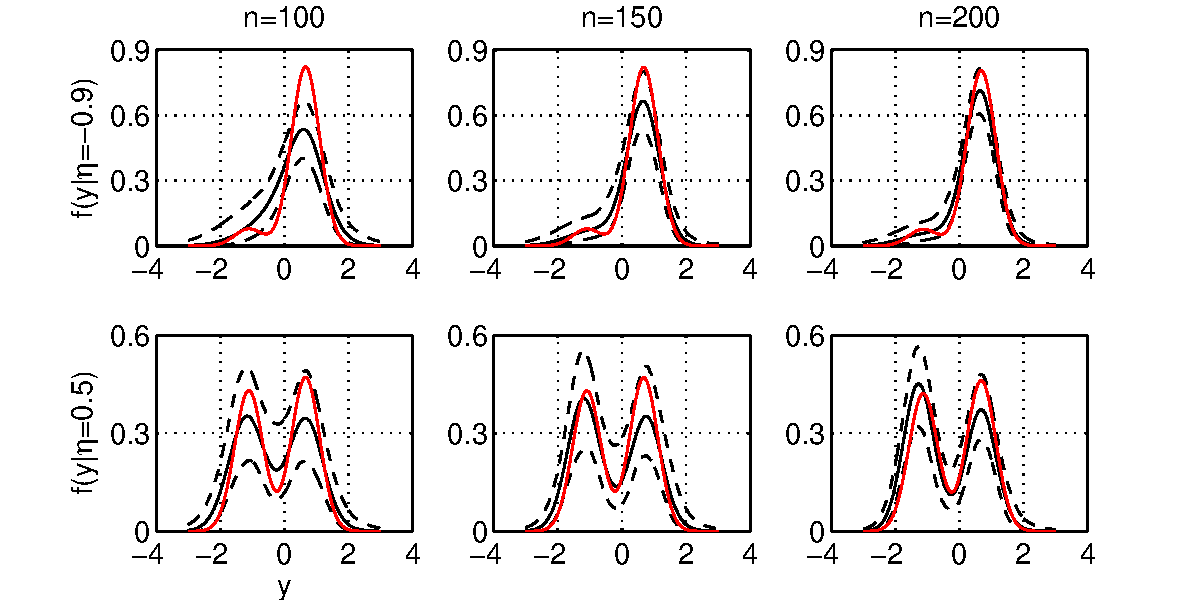
\includegraphics[width=0.5\linewidth]{../figs/density_estimates.pdf}% picture filename
  \caption{Illustrative example of model (1) suggesting that our posterior estimates of the conditional density are converging as $n$ increases even when $F_{Y|\eta}$ is highly nonlinear and $F_{X|\eta}$ is very high-dimensional.  
True (red) and estimated (black) density ($50$th percentile: solid line, $2.5$th and $97.5$th percentiles: dashed lines) for two data positions along the manifold (top panels: $\eta \approx -0.9$,  bottom panels: $\eta \approx 0.5$) considering different training set sizes.}\label{plotDensity}
\end{SCfigure}
\vspace{-10pt}
% \begin{figure}[h!]
% \centering
%  \vskip -10pt 
% 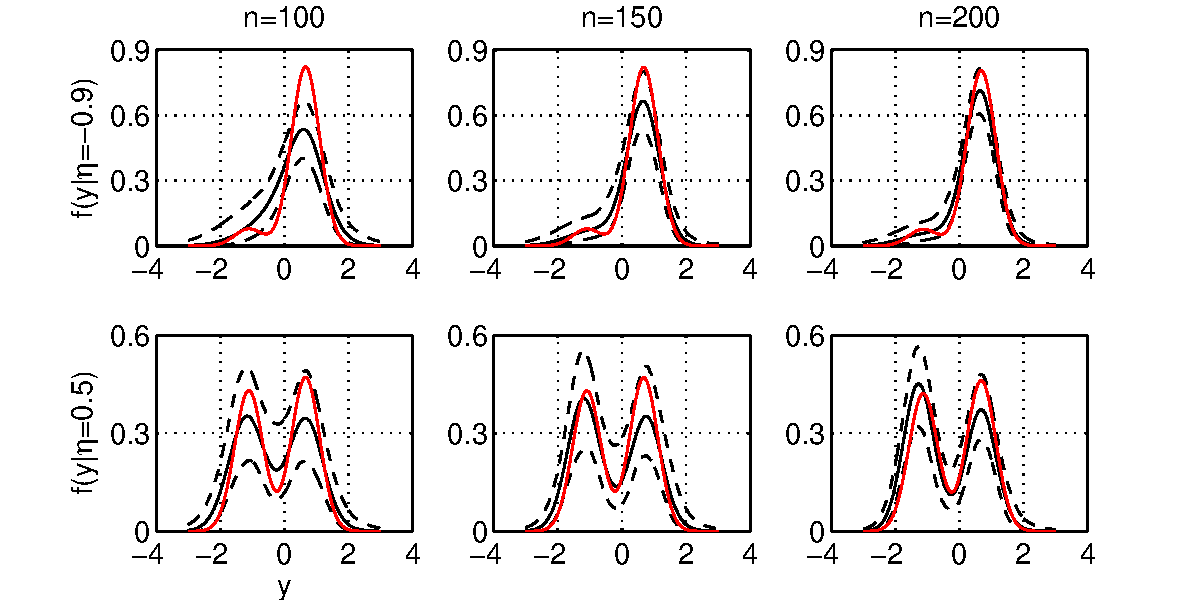
\includegraphics[width=0.8\linewidth]{../figs/density_estimates.pdf}
% \vskip -12pt 
% % 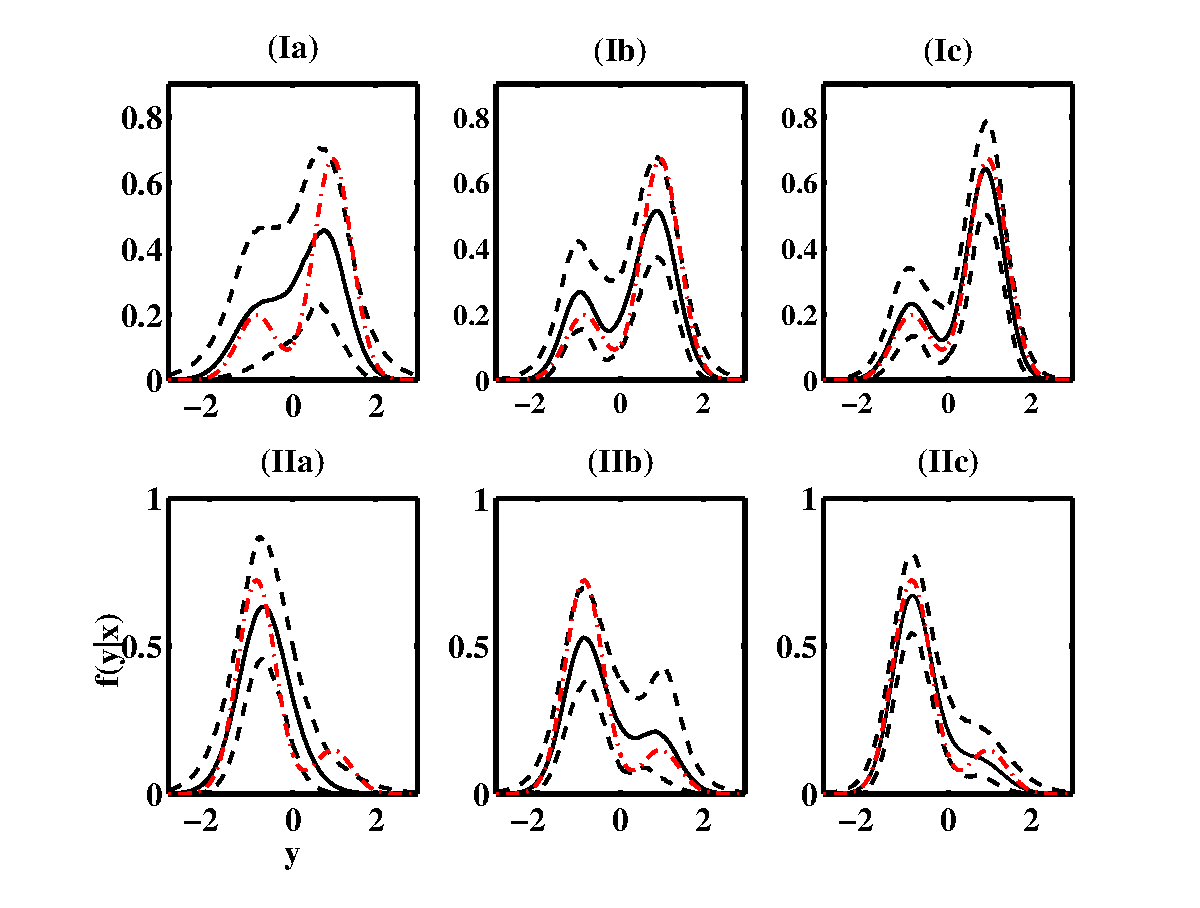
\includegraphics[width=90mm,height=80mm]{densityestimate.eps}
% \caption{Illustrative example suggesting that our posterior estimates of the conditional density are converging as $n$ increases even when $F_{Y|\eta}$ is highly nonlinear and $F_{X|\eta}$ is very high-dimensional.  We simulated data according to model (1) with parameters $(\mu_1,\sigma_1)=(-2,1)$, $(\mu_2,\sigma_2)=(2,1)$, $\sigma_x=0.01$, and $c=20$ for different sample sizes. True (red) and estimated (black) density ($50$th percentile: solid line, $2.5$th and $97.5$th percentiles: dashed lines) for two data positions along the manifold (top panels: $\eta \approx -0.9$,  bottom panels: $\eta \approx 0.5$) considering different training set size. } \label{plotDensity}
% \vskip -20pt 
% \end{figure}




\subsection{Quantitative Comparisons for Simulated Data} \label{sub:sim}

Figure \ref{fig:boxplots} compares the numerical performance of our algorithm (MSB) with Lasso (black), CART (red), and PC regression (green) in terms of both mean-squared error (top) and CPU time (bottom) for models (2), (3), and (4) in the left, middle, and right panels respectively. These figures show relative performance on a \emph{per simulation basis}, thus enabling a much more powerful comparison than averaging performance for each algorithm over a set of simulations.  Note that these three simulations span a wide range of models, including
nonlinear smooth manifolds such as the swissroll (model 2),
relatively simple linear subspace manifolds (model 3), 
and a union of linear subspaces model (model 4).

In terms of predictive accuracy, the top panels show that for all three simulations,  in every dimensionality that we considered---including $p = 0.5 \times 10^6$---MSB is more accurate than either Lasso, CART, or PC regression.  Note that this is the case even though MSB provides much more information about the posterior $F_{Y|X}$, yielding an entire posterior over $F_{Y|X}$, rather than merely a point estimate.

In terms of computational time, MSB is much faster than the competitors for large $p$ and $n$, as shown in the bottom three panels.  The supplementary materials show that computational time for MSB is relatively constant as a function of $p$, whereas Lasso's computational time grows considerably with $p$.  Thus, for large enough $p$, MSB is significantly faster that Lasso.  MSB is faster than CART and PC regression for all $p$ and $n$ under consideration.  Thus, it is clear from these simulations that MSB has better scaling properties---in terms of both predictive accuracy and computational time---than the competitor methods. 



\begin{figure}[h!]
\centering
 \vskip -20pt 
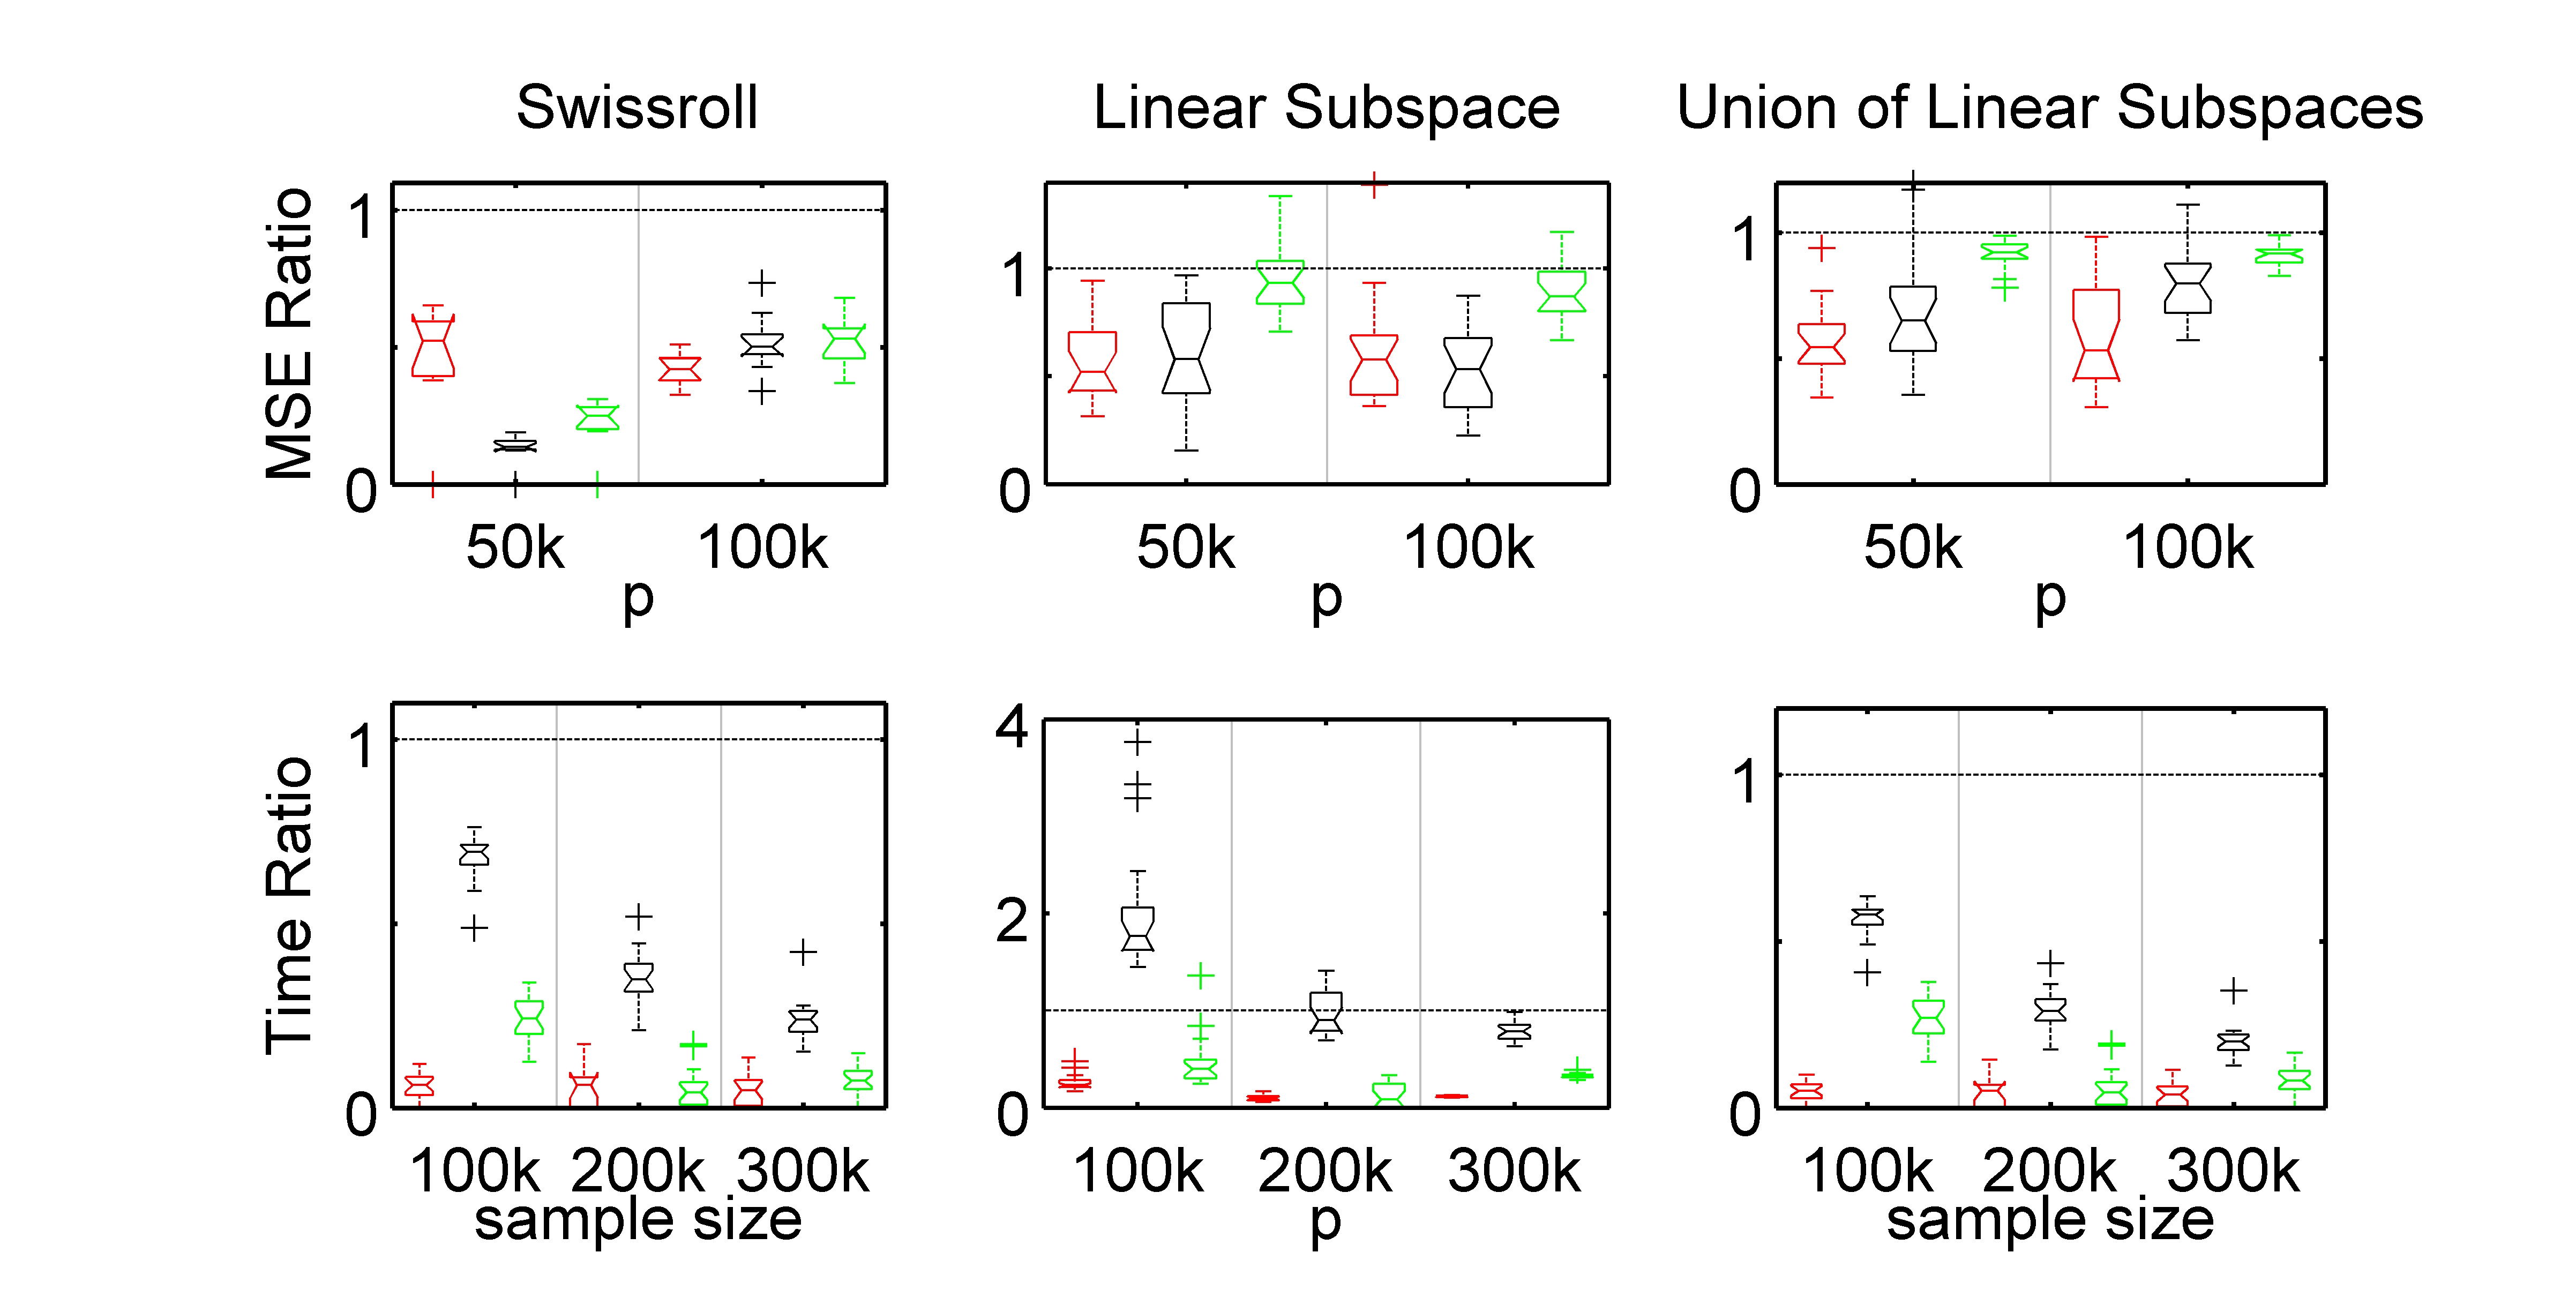
\includegraphics[width=1.0\linewidth]{../figs/boxplots.png}
% 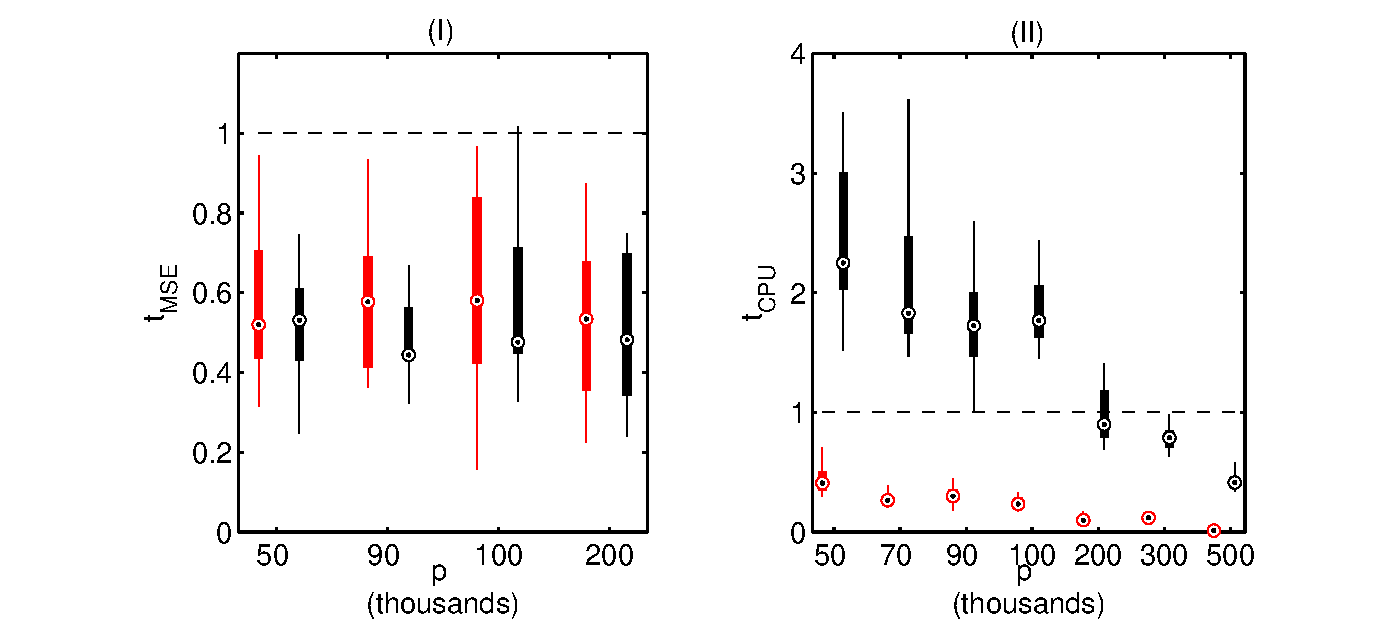
\includegraphics[width=.6\linewidth]{../figs/experiment1.eps} 
% 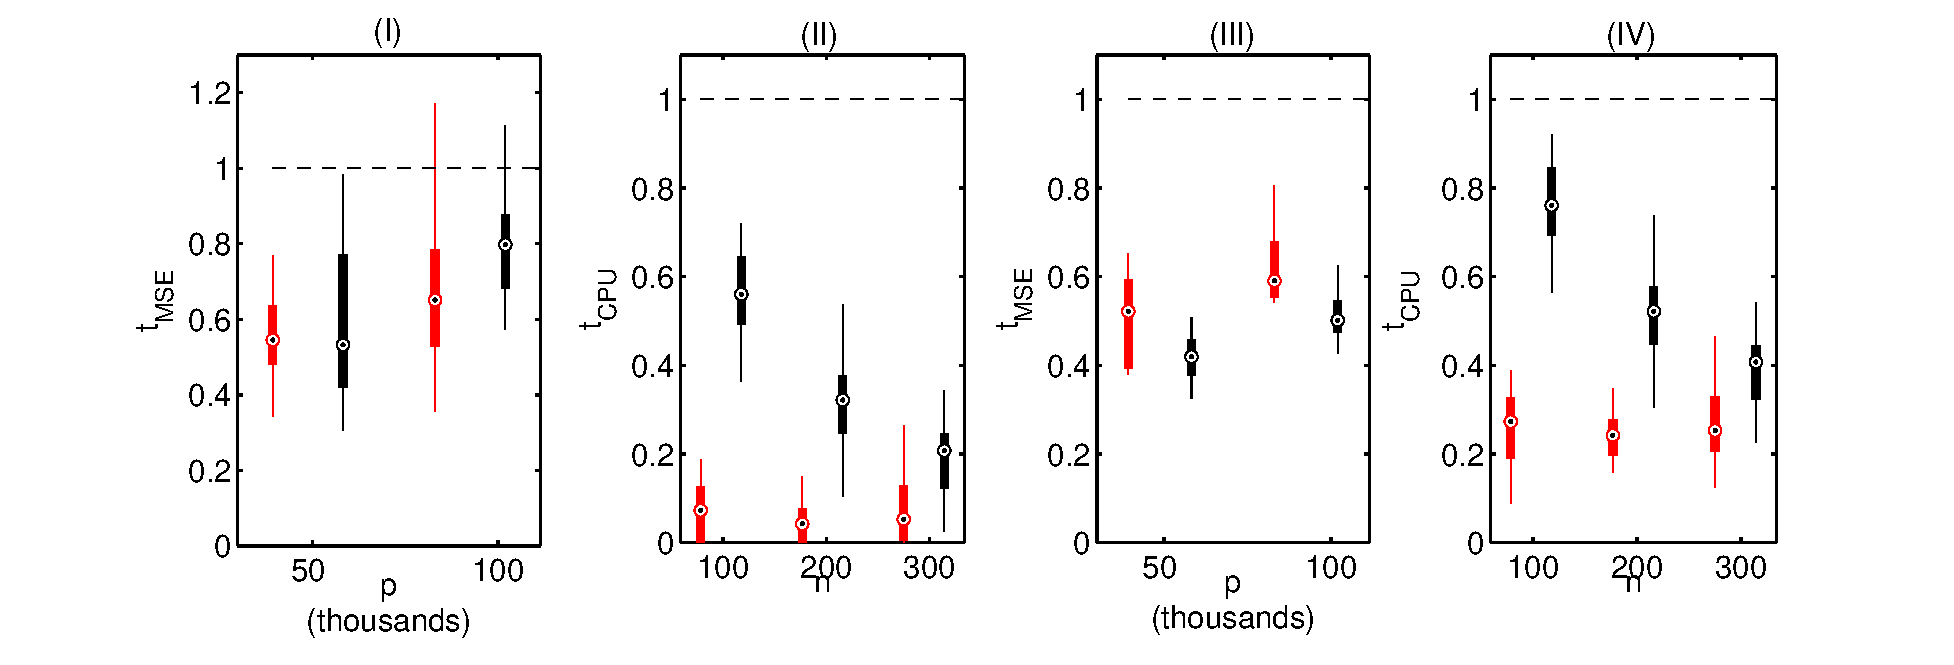
\includegraphics[width=0.8\linewidth]{../figs/nonlinear.eps} 
 \vskip -10pt 
\caption{
Numerical results for various simulation scenarios.  Top plots depict the relative mean-squared error of MSB (our approach), versus CART (red), Lasso (black), and PC regression (green) for as a function of ambient dimension of $x$.  
Bottom plots depict the ratio of CPU time as a function of sample size.
The three simulation scenarios are: 
swissroll (left),
linear subspaces (middle), 
union of linear subspaces (right). 
MSB outperforms both CART, Lasso, and PC regression in all three scenarios regardless of ambient dimension ($r_{mse}^{\mc{A}}< 1$ for all $p$).  MSB compute time is relatively constant as $n$ or $p$ increase, whereas Lasso's compute time increases, thus, as $n$ or $p$ increase, MSB CPU time becomes less than Lasso's.  MSB was always significantly faster than CART and PC regression, regardless of $n$ or $p$.  For all panels, $n=100$ when $p$ varies, and $p=300\,000$ when $n$ varies. k indicates $1000$, e.g., $100$k$=10^5$.
} 

\label{fig:boxplots}
\end{figure}

 



\subsection{Quantitative Comparisons for Neuroscience Applications} \label{sub:real}



Table \ref{real} shows the mean and standard deviation of point-estimate predictions per subject (using leave-one-out) for the two neuroscience applications that we investigated: (i) predicting creativity from diffusion MRI (creativity) and, (ii) predicting head motion based on functional MRI (movement).  For the creativity application, $p$ was relatively small, ``merely'' $2,415$, so we could run Lasso, CART, and random forests (RF) \cite{Brieman2001}.  For the movement application, $p$ was nearly one million. 

For both applications, MSB yielded improved predictive accuracy over all competitors.  Although CART and Lasso both yielded better performance on the relatively low-dimensional predictor example (creativity), their computational scaling was poor, such that CART yielded a memory fault on the higher-dimensional case, and Lasso required substantially more time than MSB.  







\begin{table}[t]
\caption{Neuroscience application quantitative performance comparisons. Squared error predictive accuracy per subject (using leave-one-out) was computed. we report the mean and standard deviation (s.d.) across subjects of squared error, as well as CPU time (in seconds).
We compare multiscale stick-breaking (MSB), CART, Lasso, random forest (RF), and PC regression. MSB outperforms all the competitors in terms of predictive accuracy and scalability for both applications.  Only MSB and Lasso even ran for the $\approx 10^6$ dimensional application.}\label{real}
\vskip 0.15in
\begin{center}
\begin{small}
\begin{sc}
\begin{tabular}{llcccccccc}
\hline
data &$n$&$p$ &model&mse (s.d.) & time (s.d.) \\ %$r_{T}$ & $r_{M}$ & $r_{V}$\\
\hline
creativity & 108 & 2,415 & MSB &$0.56 \, (\dd{??})$ &  $1.1 \, (0.02)$\\
 &&& CART & $1.10 \, (\dd{??}) $ &  $0.9 \, (0.01)$\\
&&& Lasso & $0.63 \, (\dd{??})$  &  $0.40 \, (0.10)$\\
&&& RF & $0.57 \, (\dd{??})$ &   $78.2 \, (0.59)$\\
&&& PC regression & \dd{??,  (??)} & \dd{?? , (??)}
\\
\hline
 movement & 56 & $\approx 10^6$& MSB &$0.76 \, (\dd{??})$  & $20.98 \, (2.31)$\\
 &&& Lasso & $1.02 \, (\dd{??})$ & $96.18 \, (9.66)$\\
% &&& PC regression & \dd{??,  (??)} & \dd{?? , (??)}\\
\hline
\end{tabular}
\end{sc}
\end{small}
\end{center}
\vspace{-15pt}
\end{table}

\section{Discussion} \label{sec:disc}

In this work we have introduced a general formalism to estimate conditional distributions via  multiscale dictionary learning.  An important property of any such strategy is the ability to scale up to ultrahigh-dimensional predictors.  We considered simulations and real-data examples where the dimensionality of the predictor space exceeded several hundred thousand.  To our knowledge, no other approach to learn conditional distributions can run at this scale.  Our approach explicitly assumes that the posterior $F_{Y|X}$ can be well approximated by projecting $X$ onto a lower-dimensional space, $F_{Y|X} \approx F_{Y|\eta}$, where $\eta \in \mc{M} \subset \Real^d$, and $x \in \Real^d$.   Note that this assumption is much less restrictive than assuming that $X$ is close to a low-dimensional space; rather, we only assume that the part of $F_X$ that ``matters'' to predict $Y$ lives near a low-dimensional subspace.  Because a fully Bayesian strategy remains computationally intractable at this scale, we developed a pseudo-Bayesian approach, fixing the partition tree, but integrating over scales and posteriors.

We demonstrate that even though we obtain posteriors over the conditional distribution $F_{Y|X}$, our approach, dubbed multiscale stick-breaking (MSB), outperforms several standard machine learning algorithms in terms of both predictive accuracy and computational time, as the sample size ($n$) and ambient dimension ($p$) increase.  This improvement was demonstrated when the $\mc{M}$ was a swissroll, a latent subspace, a union of latent subspaces, and real data (for which the latent space may not even exist).    

In future work, we will extend these numerical results this Bayesian theory.  Indeed, while multiscale methods benefit from a rich theoretical foundation \cite{Allard2012}, the relative advantages and disadvantages of a fully Bayesian approach, in which one can estimate posteriors over all functionals of $F_{Y|X}$ at all scales, remains relatively unexplored.  

% \clearpage
\bibliographystyle{unsrt} 
\bibliography{nipsMSB} 


\end{document}



































